\subsection{Simulated Annealing} \label{subsec:Grundlagen_SimulatedAnnealing}

Eine an der Physik, nämlich an der Metallurgie, orientierte Metaheuristik stellt \acf{SA} (dt. simuliertes Abkühlen) dar und wurde von den 3 IBM Wissenschaftlern Kirkpatrick, Gelatt und Vecchi im Jahre 1992 vorgeschlagen und im Jahr 1993 veröffentlicht. \cite[vgl.][S. 19]{siarry_metaheuristics_2016} \\

Für einen gegebenen Körper gilt es, nachdem dem Körper eine sehr hohe Temperatur zugeführt wurde, einen energetisch günstigen Zustand zu erreichen. Durch das Erhöhen der Temperatur zu einem sehr hohen Punkt wird die Struktur des Körpers zunächst geschmolzen. Der Körper befindet sich somit in einer flüssigen Phase, in welcher die Partikel des Körpers zufällig verteilt sind. Der Körper wird über das Abkühlen gemäß eines besonderen Temperaturschemas wieder in eine stabile Phase zurückgeführt und erreicht somit einen energetisch günstigen Zustand. Sowohl die initiale Temperatur als auch die Kühlungszeit müssen eine entsprechende Höhe aufweisen, da ansonsten ein metastabiler Zustand erreicht wird, in welcher die Energie nicht minimal ist. Der Prozess wird Härtung genannt, wenn die Temperaturabnahme nicht stetig ist und durch eine abrupte Abkühlung beeinflusst wird. Die Funktionsweisen und die Unterschiede zwischen dem Härtungs- und dem Abkühlungsprozess lassen sich über die Abbildung \ref{img:simulatedannealing_realworld} visualisieren. \cite[vgl.][S. 2 f.]{gendreau_handbook_2019} 

\begin{figure}[H]
    \centering
    \noindent\makebox[\textwidth]{%
    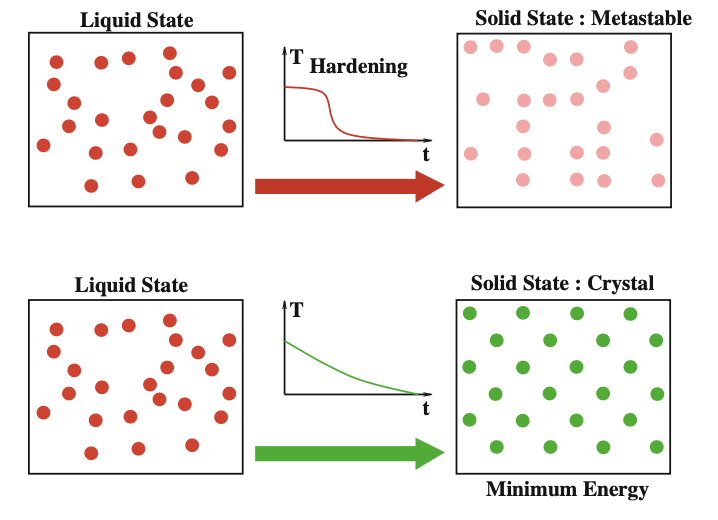
\includegraphics[width=0.48\textwidth]{assets/img/02_Grundlagen/SimulatedAnnealing_RealWorld.png}
    }
    \caption{Funktionsweise der Abkühlungs- und Härtungsprozesse} 
    \label{img:simulatedannealing_realworld}
    \source{\cite[][S. 3]{gendreau_handbook_2019} }
\end{figure}

Zwischen einem Optimierungsproblem und dem physikalischen System lassen sich Analogien ziehen. In der Physik wird die freie Energie betrachtet, bei dem Optimierungsproblem die Zielfunktion. Die Positionierung der Partikel stellt die Analogie zu den Parametern eines Problems dar. Das Ziel innerhalb eines physikalischen System liegt darin, dass ein energiearmer Zustand erreicht wird. Dies trifft ebenfalls bei Optimierungsproblemen zu, bei welchen Konfigurationen gesucht werden, welche als \glqq gut\grqq{} klassifiziert werden können oder im besten Fall am optimalsten sind. \cite[vgl.][S. 20]{siarry_metaheuristics_2016} 

\begin{lstlisting}[caption={Simulated Annealing (Quelle: \cite[vgl.][S. 714]{hosseinabadi_novel_2017}}), label=lst:simulatedannealing, mathescape=truexinputencoding={utf8}, extendedchars=false, escapeinside=``]
Create an initial solution $s$ inside the search space;
Select initial temperatur $T_0$;
Select rate of temperature decrease $\alpha \in [0.80, 0.99]$;
$T \leftarrow T_0$;  
while stopping criteria not satisfied do
    Select random solution $s' \in N(s)$;
    if f(s') < f(s)
        $s \leftarrow s'$;
    else
        $\Delta \leftarrow f(s') < f(s)$; 
        if random(0, 1) $< \exp(- \dfrac{\Delta}{T}$)
            $s \leftarrow s'$;
    $T \leftarrow T * \alpha$;
end
return the best solution;
\end{lstlisting}

Innerhalb des Algorithmus aus Listing \ref{lst:simulatedannealing} wird zunächst eine initiale Temperatur $T_0$ ausgewählt. Die Senkung anhand eines Temperaturschemas wird über eine Temperatursenkungsrate $\alpha \in [0.80, 0.99]$ realisiert. Wie auch bei der \ac{LS} wird eine initiale Lösung $s$ benötigt, welche zufällig oder über Heuristiken erzeugt werden können. Die initiale Lösung und Temperatur entsprechen dem flüssigen Zustand im Abkühlungsprozess. Nach jeder Iteration innerhalb des Algorithmus wird die Temperatur mit der Temperatursenkungsrate multipliziert $T \leftarrow T * \alpha$, was nach jeder Iteration zu einer Senkung der Temperatur führt. Um die Analogie zur Verfestigung zu realisieren, nutzt der Algorithmus die Nachbarschaftsfunktion, um so eine zufällige Lösung $s'$ auszuwählen. Über die Nutzung einer Akzeptanzfunktion gemäß Formel \ref{align:sa_acceptance} \cite[vgl.][S. 6]{gendreau_handbook_2019} und das Generieren einer zufälligen Zahl $r \in [0, 1]$ wird die Akzeptanz der Lösung $s'$ bestimmt. Sofern $r \leq P(s, s')$ gilt, wird die aktuelle Lösung überschrieben $s \leftarrow s'$. Das Annehmen von verschlechternden Lösungen im Algorithmus trägt maßgeblich zur Erkundung des Suchraums bei. Die Akzeptanz von schlechteren Lösungen sinkt über die Iterationen, da die ebenfalls sinkende Temperatur maßgebend zum Akzeptanzwert ist. Eine sinkende Temperatur impliziert, dass die Partikel innerhalb eines physikalischen Systems sich weniger stark bewegen. Gänzlich werden bei einer Temperatur $T \approx 0$ schlechtere Lösungen abgelehnt, was dazu führt, dass der Algorithmus lediglich als lokale Suche agiert. Es werden dann nur Lösungen angenommen, wenn die selektierte Lösung aus der Nachbarschaft besser als die aktuelle ist. \cite[vgl.][S. 5 f.]{gendreau_handbook_2019} \cite[vgl.][S. 21 f.]{siarry_metaheuristics_2016} 

\begin{align}
P(s, s') = \left\{\begin{array}{ll} 
        1 & \text{wenn $f(s') < f(s)$} \\
        e^{\Big(\dfrac{f(s) - f(s')}{T}\Big)} & \text{sonst} \\
     \end{array}\right. \label{align:sa_acceptance}
\end{align}

Wie bei der \ac{TS} stehen beim \ac{SA} unterschiedliche Stopkriterien zur Verfügung. Der Algorithmus von \cite[][S. 6 f.]{gendreau_handbook_2019} iteriert solange, bis die Temperatur bei $T \approx 0$ liegt. Der Algorithmus von \cite[][S. 714]{hosseinabadi_novel_2017} nutzt zusätzlich eine feste Anzahl an Iterationen, die durchlaufen werden müssen. Alternativ können die aus dem Abschnitt \ref{subsec:Grundlagen_TabuSearch} für die \ac{TS} vorgestellten Kriterien verwendet werden. Ein weitere Besonderheit stellt die Verwendung einer Boltzmann Konstante $k_B$ dar, welche zur Gewichtung der Temperatur in der Annahmefunktion beiträgt \cite[vgl.][S. 21]{siarry_metaheuristics_2016}. Durch die Verwendung einer Boltzmann Konstante $k_B$ lässt sich die Relevanz der Temperatur bei der Akzeptanzfunktion verändern.  
